%!TEX root = ../../report.tex
\section{Feature Map for Monte Carlo Localization}
\label{sec:localzation_feature_map}
The desired features for AMCL are static objects. 
This could be objects like walls and heavy machinery which never move.  
The elements added for the localization should therefore be cells that have been very static. 
In the interpretation step each cell is classified as static occupied or not. 
The parameters available for classification are:
\begin{itemize} 
\item Sum of state scores for occupied
\item Sum of state scores for free
\item Sum of event scores for exit
\item Sum of event scores for entry
\item Previous observation
\item \(\hat{\lambda}_{exit}\) - estimated by exit event and occupied state scores
\item \(\hat{\lambda}_{entry}\) - estimated by entry event and free state scores
\end{itemize}

We propose a simple classifier that bases its decisions on \(\lambda_{exit}\) and the ratio between sum of sate scores for both occupied and free as shown in equation \ref{eq:classifier}. 
Cells that have been classified as static occupied are given a lethal cost in the costmap. Alternatively the cost is assigned the Markov projection cost $\kappa$ described in section \ref{sec:cost_interpretation_path_planning}. 

\begin{equation}
\label{eq:classifier}
c_i = 
\begin{cases}
lethal, & \text{if } \lambda_{exit}(i) < l_{exit} \land \frac{s_{score}^{occ}(i)}{s_{score}^{free}(i)}  > l_{occ}
\\
\kappa, & \text{otherwise}
\end{cases}
\end{equation}
%l exit  = 0.15     l occ = 2

$l_{exit}$ is set to $0.15$ because one of the primary attributes of static obstacles is that the probability for them disparaging is very low.
$l_{occ}$ is set to $2$ to ensure that the cells has been more occupied than free. 
The classification was determined based on simulation as well as real world data.
The simulation setup is identical to the setup used in section \ref{sec:fremen_sim_eval}. 
In the simulation the robot drove from the top-right corner to the bottom-left. This means that the amount of data from the two remaining corners are very limited.

Figure \ref{fig:amcl_classifier} shows the classification results as well as the ground truth. 
Figure \ref{fig:amcl_classifier:worst} shows a bad classifier that includes all the dynamic obstacles. 
The results from the chosen classifier are shown in figure \ref{fig:amcl_classifier:chosen}. In the result, almost all of the dynamic obstacles are removed. It was not possible to adjust the limits $l$ to suppress the remaining dynamic obstacles without damaging the true walls.
%
%
%% FIGURE - CLASSIFICATIONS
\begin{figure}[htbp]
	\label{fig:amcl_classifier}
	\begin{subfigure}[t]{0.3\linewidth}
		\centering
		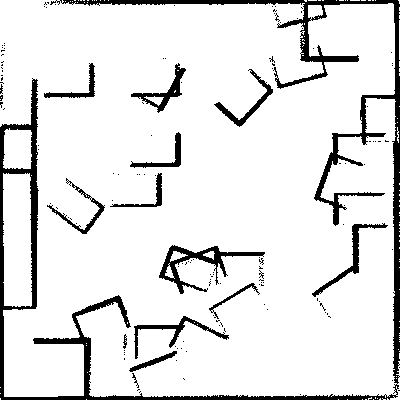
\includegraphics[width=1\linewidth]{chapters/cost_interpretation/figures/occ_above_0_classifier.png}
		\caption{Obstacles: $l_{exit} = 1$ and $l_{occ} = 1$}
		\label{fig:amcl_classifier:worst}
	\end{subfigure}
	\hspace*{\fill}
	\begin{subfigure}[t]{0.3\linewidth}
		\centering
		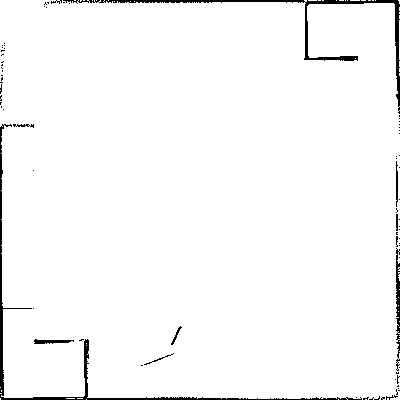
\includegraphics[width=1\linewidth]{chapters/cost_interpretation/figures/chosen_classifier.png}
		\caption{Obstacles: $l_{exit} = 0.15$ and $l_{occ} = 2$}
		\label{fig:amcl_classifier:chosen}
	\end{subfigure}
	\hspace*{\fill}
	\begin{subfigure}[t]{0.3\linewidth}
		\centering
		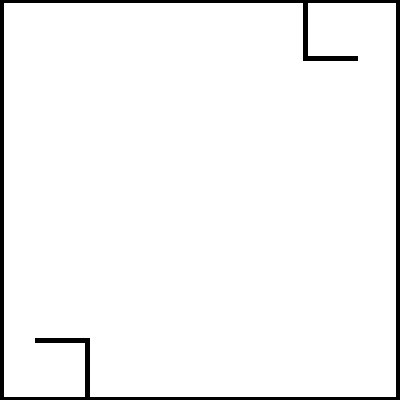
\includegraphics[width=1\linewidth]{chapters/cost_interpretation/figures/dynamic_area_web.png}
		\caption{Ground truth map}
		\label{fig:amcl_classifier:groundtruth}
	\end{subfigure}
	\caption{Costmap generated with different classifiers and the ground truth. Obstacles are shown in black.}
    \label{fig:amcl_classifier}
\end{figure}


\begin{figure}
\centering
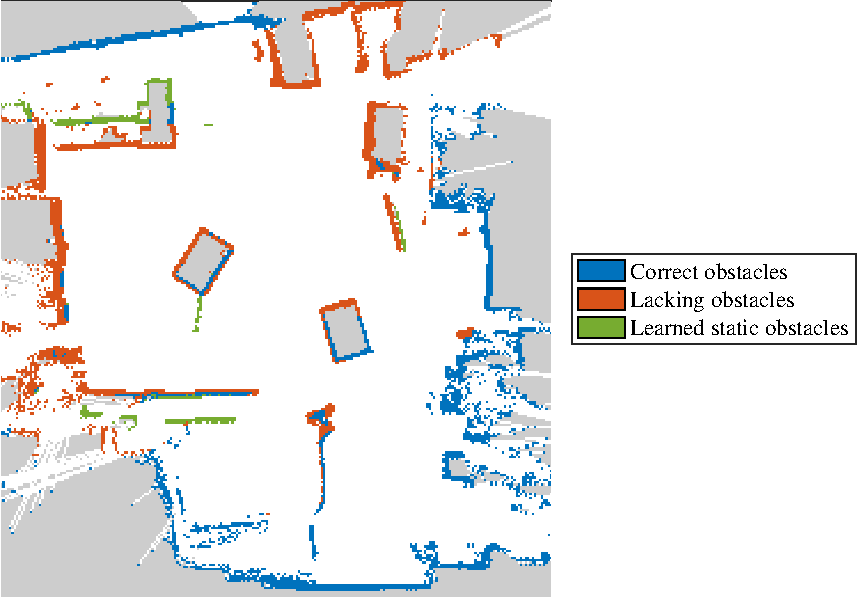
\includegraphics[scale=1]{chapters/evaluation/figures/static_classified_localization_test-crop}
\caption{}
\label{fig:static_classified_localization_test-crop}
\end{figure}
